\documentclass[../main.tex]{subfiles}

\begin{document}

    \begin{table}[H]
        \begin{center}
            \begin{tabular}{| p{8cm}| p{8cm}|}
                \hline
                \multicolumn{2}{|c|}{    \textbf{Modele procesu testowego}}\\
                \hline
                \textbf{TMAP lifecycle model} &  \textbf{ISO 29119}\\
                \hline

                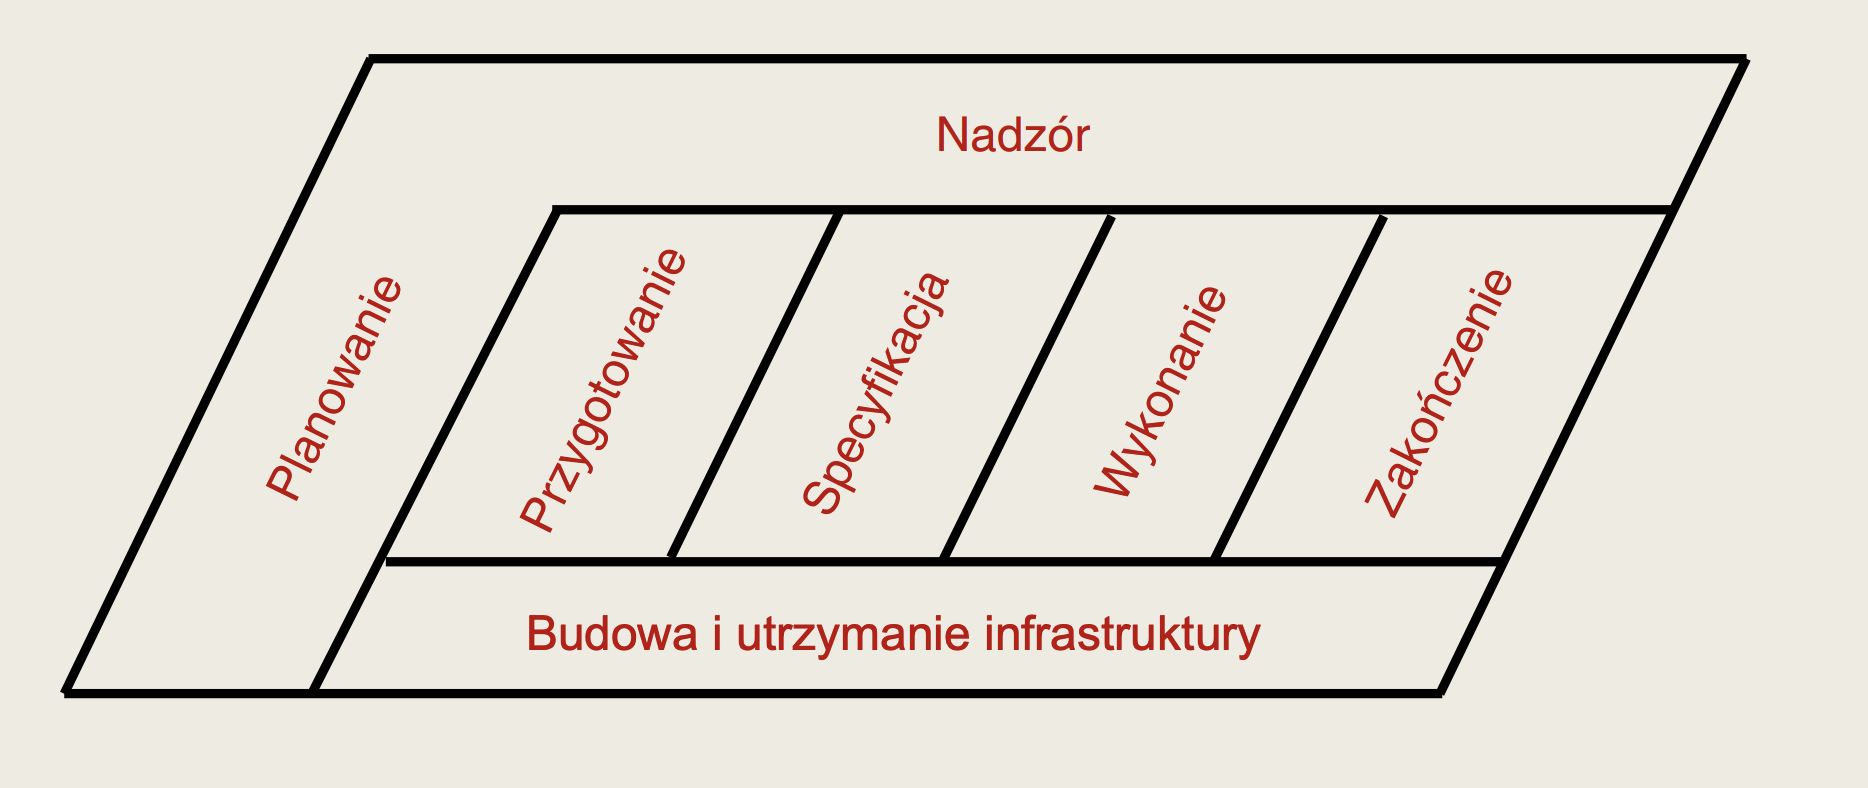
\includegraphics[width=8cm]{tmap.png}

                Proces jest \textbf{generyczny}, tzn. może być stosowany do wszystkich
                poziomów i typów testów. Każda faza dzieli się na określone czynności.
                &

                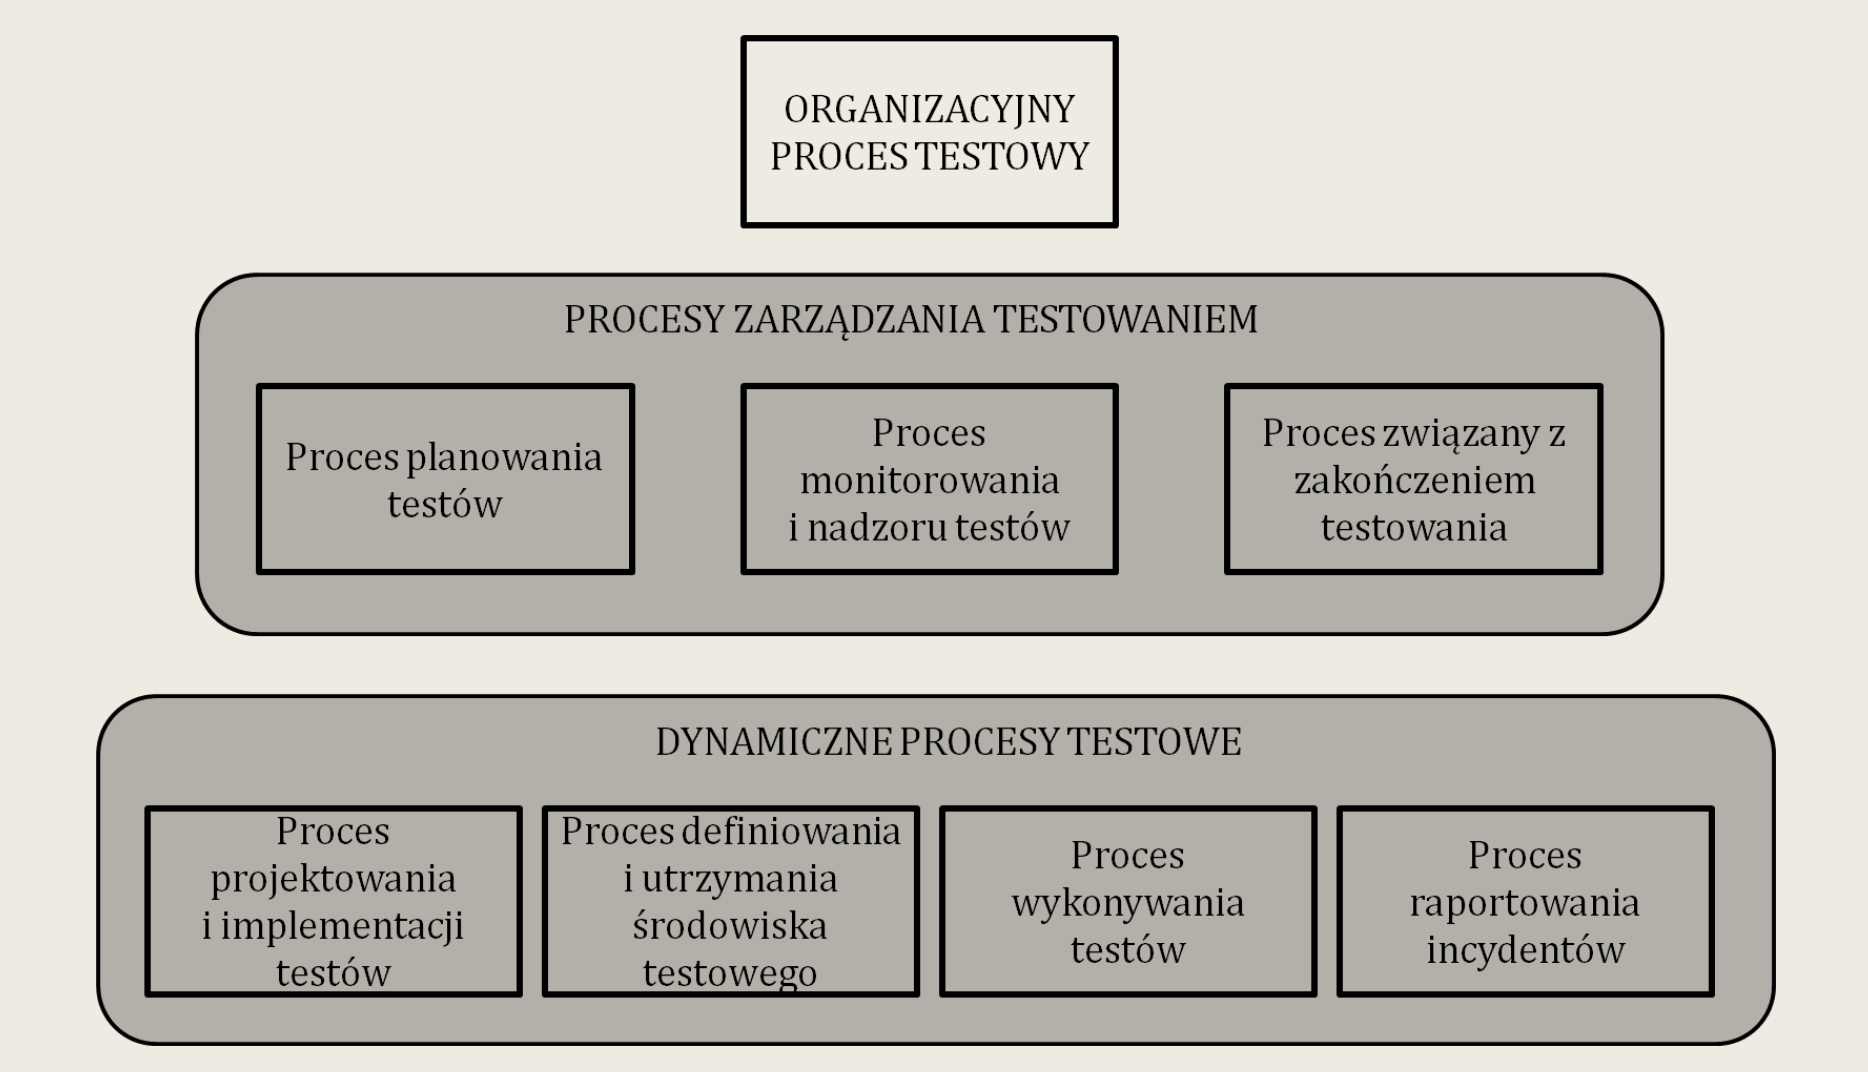
\includegraphics[width=8cm]{iso29119.png}\\

                \hline

            \end{tabular}
        \end{center}
    \end{table}

    \subsection{Poziomy testów.}

    \textbf{Poziom testów} określa \textbf{sposób} testowania ze względu na \textbf{postać}
    testowanego obiektu w kontekście cyklu życia (\textbf{co testujemy?}).


    \begin{table}[H]
        \begin{center}
            \begin{tabular}{| p{8cm}| p{8cm}|}
                \hline
                \multicolumn{2}{|c|}{ \textbf{TESTY JEDNOSTKOWE}}\\
                \hline
                \textbf{Podstawa testów} & wymagania na moduły, projekt szczegółowy, kod\\
                \hline
                \textbf{Typowe obiekty} & moduły, programy, funkcje, klasy, procedury\\
                \hline
            \end{tabular}
        \end{center}
    \end{table}

    \begin{table}[H]
        \begin{center}
            \begin{tabular}{| p{8cm}| p{8cm}|}
                \hline
                \multicolumn{2}{|c|}{ \textbf{TESTY INTEGRACYJNE}}\\
                \hline
                \textbf{Podstawa testów} & projekt systemu, architektura, przypadki użycia\\
                \hline
                \textbf{Typowe obiekty} & interfejsy, podsystemy, konfiguracje systemów\\
                \hline
            \end{tabular}
        \end{center}
    \end{table}
    Strategie testów integracyjnych:
    \begin{itemize}
        \item \textbf{top-down}: testujemy moduły "w dół", w kolejności w jakiej się
        wywołują
        \item \textbf{bottom-up}: testujemy moduły od ostatniego wywoływanego
        \item \textbf{funkcjonalne}: testujemy wywołania wewnątrz funkcjonalności
        \item \textbf{sekwencja przeprowadzania transakcji}
        \item \textbf{big-bang}: wszystko integrowane i testowane naraz
    \end{itemize}
    \begin{table}[H]
        \begin{center}
            \begin{tabular}{| p{8cm}| p{8cm}|}
                \hline
                \multicolumn{2}{|c|}{ \textbf{TESTY SYSTEMOWE}}\\
                \hline
                \textbf{Podstawa testów} & wymagania na system, przypadki użycia,
                specyfikacja funkcjonalna, raporty analizy ryzyka\\
                \hline
                \textbf{Typowe obiekty} & system, podręczniki użytkownika i operatora,
                konfiguracja systemu\\
                \hline
                \hline
                \multicolumn{2}{|c|}{ \textbf{TESTY AKCEPTACYJNE}}\\
                \hline
                \textbf{Podstawa testów} & wymagania użytkownika, wymagania na system,
                przypadki użycia, procesy biznesowe, raporty
                analizy ryzyka\\
                \hline
                \textbf{Typowe obiekty} & Procesy biznesowe w pełni zintegrowanego
                systemu, procesy operacyjne i utrzymania systemu,
                procedury, raporty, dane konfiguracyjne\\
                \hline
            \end{tabular}
        \end{center}
    \end{table}
    \textbf{Typowe formy testów akceptacyjnych:}
    \begin{itemize}
        \item \textbf{testy akceptacyjne użytkownika (UAT)} – sprawdzenie gotowości do użycia
        \item \textbf{testy operacyjne (OAT)} – akceptacja przez administratora systemu (testy
        backupu, przywracania systemu, zarządzania użytkownikami, utrzymania,
        migracji danych, bezpieczeństwa itp.)
        \item \textbf{testy akceptacyjne wymagane kontraktem/regulacjami}
        \item \textbf{testy alfa, beta (polowe)}
        \begin{itemize}
            \item alfa: przeprowadzane u producenta, ale nie przez zespół deweloperski
            \item beta: przeprowadzane u klienta przez klienta/potencjalnego użytkownika
        \end{itemize}
    \end{itemize}


    \subsection{Typy testów.}

    Typ testów to zbiór czynności testowych właściwych dla weryfikacji systemu
    w oparciu o konkretny powód lub cel testów (\textbf{jak testujemy?}).

    \begin{table}[H]
        \begin{center}
            \begin{tabular}{| p{8cm}| p{8cm}|}
                \hline
                \textbf{Testowanie funkcjonalne} & \textbf{Testowanie niefunkcjonalne}\\
                \hline
                Funkcja wykonywana przez oprogramowanie - \textbf{co system robi}.
                &
                Niefunkcjonalna charakterystyka jakościowa wyrażalna ilościowo, np. niezawodność
                czy użyteczność - \textbf{jak system działa}.\\
                \hline
            \end{tabular}
        \end{center}
    \end{table}

    \begin{table}[H]
        \begin{center}
            \begin{tabular}{| p{8cm}| p{8cm}|}
                \hline
                \textbf{Testowanie strukturalne} & \textbf{Retesty i testy regresji}\\
                \hline
                \begin{itemize}
                    \item oparte na strukturze
                    \item zwykle wykonywane po testach czarnoskrzynkowych, aby sprawdzić stopień przetestowania i wyrazić go
                    ilościowo (pokrycie)
                \end{itemize}
                &
                Związany ze zmianą, tzn. potwierdzenie usunięcia defektów
                (retesty) oraz poszukiwanie niezamierzonych zmian (regresja) - \textbf{związane ze zmianami}
                \begin{itemize}
                    \item \textbf{regresja} = zjawisko pogarszania się jakości systemu na skutek
                    wprowadzanych w nim zmian
                    \item \textbf{retest} = przetestowanie naprawionego fragmentu systemu
                \end{itemize}\\

                \hline
            \end{tabular}
        \end{center}
    \end{table}


    \subsection{Statyczne techniki testowania}
    Ręczne sprawdzanie (\textbf{przeglądy}) i automatyczna analiza (\textbf{analiza statyczna}) kodu lub dokumentacji
    bez uruchamiania kodu, ale zwykle z użyciem narzędzi!

    \begin{table}[H]
        \begin{center}
            \begin{tabular}{| p{8cm}| p{8cm}|}
                \hline
                \multicolumn{2}{|c|}{ \textbf{PRZEGLĄDY}}\\
                \hline
                \textbf{Definicja} & \textbf{Korzyści z przeglądow}\\
                \hline
                \begin{itemize}
                    \item Sposoby ręcznego testowania oprogramowania (np. kodu, dokumentacji)
                    \item Pozwalają wykryć defekty wcześnie w cyklu życia (np. w wymaganiach),
                    \item Aktywność manualna, ale może być wsparta narzędziami
                \end{itemize}
                &
                \begin{itemize}
                    \item wczesne wykrycie i naprawa defektów
                    \item doskonalenie jakości tworzonego kodu
                    \item redukcja kosztu i czasu testów
                    \item mniej defektów (w późniejszych fazach)
                    \item ulepszenie komunikacji
                \end{itemize}\\
                \hline
            \end{tabular}
        \end{center}
    \end{table}

    \begin{table}[H]
        \begin{center}
            \begin{tabular}{|p{3cm}||p{8cm}|p{5cm}|}
                \hline
                \multicolumn{3}{|c|}{ \textbf{Rodzaje przeglądów}}\\
                \hline
                \textbf{Typ przeglądu} & \textbf{Charakterystyka} & \textbf{Cel}\\
                \hline
                \hline
                \textbf{nieformalny} & brak formalnego procesu, może przybrać formę programowania w parach lub nieformalnej rozmowy &
                tani sposób na osiągnięcie niewielkich korzyści\\
                \hline
                \textbf{przejrzenie} & prowadzone przez autora; opcjonalne przygotowanie przed spotkaniem,
                opcjonalny raport z przeglądu & uczenie się, zrozumienie, znajdowanie usterek\\
                \hline
                \textbf{techniczny} & przeszkolony moderator, przygotowanie przed spotkaniem, zdefiniowany proces
                postępowania & podjęcie decyzji, ocena alternatyw, szukanie usterek, rozw. probl. technicznych\\
                \hline
                \textbf{inspekcja} & przeszkolony moderator, wyróżnione role i metryki, formalny proces, przygotowanie przed
                spotkaniem, formalny proces kontroli napraw & wyszukiwanie usterek\\
                \hline
            \end{tabular}
        \end{center}
    \end{table}


    \begin{table}[H]
        \begin{center}
            \begin{tabular}{| p{8cm}| p{8cm}|}
                \hline
                \multicolumn{2}{|c|}{ \textbf{INSPEKCJE}}\\
                \hline
                \textbf{Proces} & \textbf{Role}\\
                \hline
                \begin{itemize}
                    \item Planowanie
                    \item Rozpoczęcie
                    \item Przygotowanie indywidualne
                    \item Kontrola/ocena/zapis wyników
                    \item Poprawki
                    \item Zakończenie
                \end{itemize}
                &
                \begin{itemize}
                    \item kierownik
                    \item moderator
                    \item autor
                    \item przeglądający
                    \item protokolant
                \end{itemize}\\
                \hline
            \end{tabular}
        \end{center}
    \end{table}


    \subsection{Projektowanie testów.}
    \textbf{Warunek testowy} (test condition) – \textbf{element} lub zdarzenie które może być
    \textbf{sprawdzone} przez jeden lub więcej \textbf{przypadków testowych} (np. funkcja,
    transakcja, atrybut jakościowy, element strukturalny).

    \textbf{Element pokrycia} (coverage item) – element lub zdarzenie używane jako
    \textbf{podstawa dla pokrycia testu} (np. przejście w maszynie stanów, instrukcja.

    \textbf{Przypadek testowy} - \textbf{generyczna struktura}: warunki początkowe, działanie i wynik = wejście, przetwarzanie, wyjście.
\end{document}